\documentclass[tikz, border=6pt]{standalone}
\IfFileExists{lmodern.sty}{\usepackage[T1]{fontenc}\usepackage{lmodern}}{}
\usepackage{amsmath,amssymb,bm}
\usepackage[scaled=0.95]{helvet}
\usetikzlibrary{arrows.meta, fit, backgrounds}
\definecolor{Blue}{HTML}{3A76D8}
\definecolor{Sky}{HTML}{2E9FD9}
\definecolor{Green}{HTML}{3BA55C}
\definecolor{Yellow}{HTML}{EAB531}
\definecolor{Orange}{HTML}{EE8133}
\definecolor{Pink}{HTML}{D9508E}
\definecolor{Purple}{HTML}{8459D1}
\definecolor{Gray}{HTML}{6B7280}
\definecolor{Ink}{HTML}{1F2937}
\tikzset{
  dot/.style={circle, fill, inner sep=0pt, minimum size=4.5pt},
  block/.style={/utils/exec={\colorlet{pytikzarg}{#1}}, draw=pytikzarg!78!black, fill=pytikzarg!14, rounded corners=3pt, align=center, inner sep=5pt, minimum height=8mm, minimum width=20mm},
  block/.default=Blue,
  op/.style={circle, draw, fill=white, inner sep=0pt, minimum size=5mm, font=\normalsize},
  group/.style={/utils/exec={\colorlet{pytikzarg}{#1}}, draw=pytikzarg!78!black, fill=pytikzarg!7, rounded corners=6pt, dashed, inner sep=8pt},
  group/.default=Gray,
}
\begin{document}
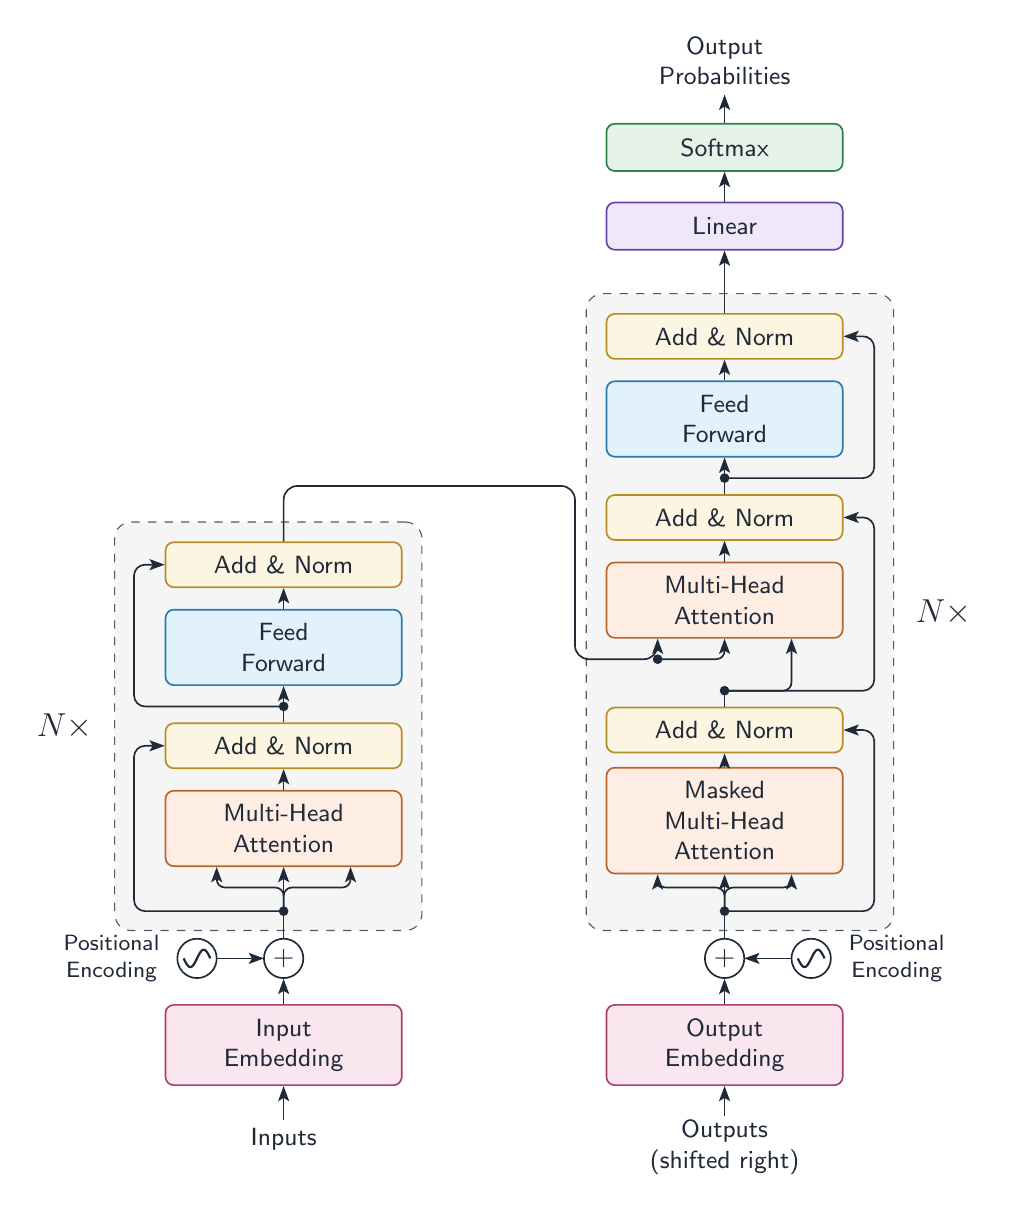
\begin{tikzpicture}[color=Ink, execute at begin picture={\sffamily}, line width=0.6pt, >={Stealth[length=5.5pt, width=4pt, inset=1.2pt]}, line join=round]
  \node[font=\small] at (0,-0.75) {Inputs};
  \node[align=center, block=Pink, minimum width=3cm, minimum height=0.9cm, font=\small] (n1) at (0,0.45) {Input\\Embedding};
  \node[op] (n2) at (0,1.55) {$+$};
  \draw[fill=white] (-1.1,1.55) circle[radius=0.25cm];
  \draw[line width=0.8pt] (-1.27,1.55) -- (-1.2613,1.5324) -- (-1.2526,1.5152) -- (-1.2438,1.4989) --
      (-1.2351,1.4839) -- (-1.2264,1.4707) -- (-1.2177,1.4595) -- (-1.209,1.4506) -- (-1.2003,1.4443)
      -- (-1.1915,1.4408) -- (-1.1828,1.4401) -- (-1.1741,1.4422) -- (-1.1654,1.4471) --
      (-1.1567,1.4547) -- (-1.1479,1.4648) -- (-1.1392,1.4771) -- (-1.1305,1.4912) -- (-1.1218,1.5069)
      -- (-1.1131,1.5237) -- (-1.1044,1.5411) -- (-1.0956,1.5589) -- (-1.0869,1.5763) --
      (-1.0782,1.5931) -- (-1.0695,1.6088) -- (-1.0608,1.6229) -- (-1.0521,1.6352) -- (-1.0433,1.6453)
      -- (-1.0346,1.6529) -- (-1.0259,1.6578) -- (-1.0172,1.6599) -- (-1.0085,1.6592) --
      (-0.9997,1.6557) -- (-0.991,1.6494) -- (-0.9823,1.6405) -- (-0.9736,1.6293) -- (-0.9649,1.6161)
      -- (-0.9562,1.6011) -- (-0.9474,1.5848) -- (-0.9387,1.5676) -- (-0.93,1.55);
  \node[align=center, anchor=east, font=\footnotesize] at (-1.45,1.55) {Positional\\Encoding};
  \draw[->] (-0.85,1.55) -- (-0.25,1.55);
  \draw[->] (0,-0.5) -- (n1.south);
  \draw[->] (n1.north) -- (n2.south);
  \node[align=center, block=Orange, minimum width=3cm, minimum height=0.95cm, font=\small] (n3) at (0,3.2) {Multi-Head\\Attention};
  \node[block=Yellow, minimum width=3cm, minimum height=0.55cm, font=\small] (n4) at (0,4.25) {Add \& Norm};
  \node[align=center, block=Sky, minimum width=3cm, minimum height=0.95cm, font=\small] (n5) at (0,5.5) {Feed\\Forward};
  \node[block=Yellow, minimum width=3cm, minimum height=0.55cm, font=\small] (n6) at (0,6.55) {Add \& Norm};
  \draw (n2.north) -- (0,2.15);
  \draw[->, rounded corners=3pt] (0,2.15) -- (0,2.45) -- (-0.85,2.45) -- (-0.85,0 |- n3.south);
  \draw[->, rounded corners=3pt] (0,2.15) -- (0,2.45) -- (0,2.45) -- (0,0 |- n3.south);
  \draw[->, rounded corners=3pt] (0,2.15) -- (0,2.45) -- (0.85,2.45) -- (0.85,0 |- n3.south);
  \node[dot, minimum size=3.5pt] at (0,2.15) {};
  \draw[->, rounded corners=4pt] (0,2.15) -- (-1.9,2.15) -- (-1.9,0 |- n4.west) -- (n4.west);
  \draw[->] (n3.north) -- (n4.south);
  \draw (n4.north) -- (0,4.75);
  \draw[->] (0,4.75) -- (n5.south);
  \node[dot, minimum size=3.5pt] at (0,4.75) {};
  \draw[->, rounded corners=4pt] (0,4.75) -- (-1.9,4.75) -- (-1.9,0 |- n6.west) -- (n6.west);
  \draw[->] (n5.north) -- (n6.south);
  \begin{scope}[on background layer]
    \node[group=Gray, fit={(n3) (n6) (-1.9,2.15)}, inner sep=7pt] (n7) {};
  \end{scope}
  \node[anchor=east, font=\large, xshift=-0.15cm] at (n7.west) {$N\times$};
  \node[align=center, font=\small] at (5.6,-0.85) {Outputs\\(shifted right)};
  \node[align=center, block=Pink, minimum width=3cm, minimum height=0.9cm, font=\small] (n8) at (5.6,0.45) {Output\\Embedding};
  \node[op] (n9) at (5.6,1.55) {$+$};
  \draw[fill=white] (6.7,1.55) circle[radius=0.25cm];
  \draw[line width=0.8pt] (6.53,1.55) -- (6.5387,1.5324) -- (6.5474,1.5152) -- (6.5562,1.4989) --
      (6.5649,1.4839) -- (6.5736,1.4707) -- (6.5823,1.4595) -- (6.591,1.4506) -- (6.5997,1.4443) --
      (6.6085,1.4408) -- (6.6172,1.4401) -- (6.6259,1.4422) -- (6.6346,1.4471) -- (6.6433,1.4547) --
      (6.6521,1.4648) -- (6.6608,1.4771) -- (6.6695,1.4912) -- (6.6782,1.5069) -- (6.6869,1.5237) --
      (6.6956,1.5411) -- (6.7044,1.5589) -- (6.7131,1.5763) -- (6.7218,1.5931) -- (6.7305,1.6088) --
      (6.7392,1.6229) -- (6.7479,1.6352) -- (6.7567,1.6453) -- (6.7654,1.6529) -- (6.7741,1.6578) --
      (6.7828,1.6599) -- (6.7915,1.6592) -- (6.8003,1.6557) -- (6.809,1.6494) -- (6.8177,1.6405) --
      (6.8264,1.6293) -- (6.8351,1.6161) -- (6.8438,1.6011) -- (6.8526,1.5848) -- (6.8613,1.5676) --
      (6.87,1.55);
  \node[align=center, anchor=west, font=\footnotesize] at (7.05,1.55) {Positional\\Encoding};
  \draw[->] (6.45,1.55) -- (5.85,1.55);
  \draw[->] (5.6,-0.45) -- (n8.south);
  \draw[->] (n8.north) -- (n9.south);
  \node[align=center, block=Orange, minimum width=3cm, minimum height=1.15cm, font=\small] (n10) at (5.6,3.3) {Masked\\Multi-Head\\Attention};
  \node[block=Yellow, minimum width=3cm, minimum height=0.55cm, font=\small] (n11) at (5.6,4.45) {Add \& Norm};
  \node[align=center, block=Orange, minimum width=3cm, minimum height=0.95cm, font=\small] (n12) at (5.6,6.1) {Multi-Head\\Attention};
  \node[block=Yellow, minimum width=3cm, minimum height=0.55cm, font=\small] (n13) at (5.6,7.15) {Add \& Norm};
  \node[align=center, block=Sky, minimum width=3cm, minimum height=0.95cm, font=\small] (n14) at (5.6,8.4) {Feed\\Forward};
  \node[block=Yellow, minimum width=3cm, minimum height=0.55cm, font=\small] (n15) at (5.6,9.45) {Add \& Norm};
  \draw (n9.north) -- (5.6,2.15);
  \draw[->, rounded corners=3pt] (5.6,2.15) -- (5.6,2.45) -- (4.75,2.45) -- (4.75,0 |- n10.south);
  \draw[->, rounded corners=3pt] (5.6,2.15) -- (5.6,2.45) -- (5.6,2.45) -- (5.6,0 |- n10.south);
  \draw[->, rounded corners=3pt] (5.6,2.15) -- (5.6,2.45) -- (6.45,2.45) -- (6.45,0 |- n10.south);
  \node[dot, minimum size=3.5pt] at (5.6,2.15) {};
  \draw[->, rounded corners=4pt] (5.6,2.15) -- (7.5,2.15) -- (7.5,0 |- n11.east) -- (n11.east);
  \draw[->] (n10.north) -- (n11.south);
  \draw (n11.north) -- (5.6,4.95);
  \node[dot, minimum size=3.5pt] at (5.6,4.95) {};
  \draw[->, rounded corners=4pt] (5.6,4.95) -- (7.5,4.95) -- (7.5,0 |- n13.east) -- (n13.east);
  \draw[->, rounded corners=3pt] (5.6,4.95) -- (6.45,4.95) -- (6.45,0 |- n12.south);
  \draw[->, rounded corners=5pt] (n6.north) -- (0,7.55) -- (3.7,7.55) -- (3.7,5.35) -- (4.75,5.35) --
      (4.75,0 |- n12.south);
  \node[dot, minimum size=3.5pt] at (4.75,5.35) {};
  \draw[->, rounded corners=3pt] (4.75,5.35) -- (5.6,5.35) -- (5.6,0 |- n12.south);
  \draw[->] (n12.north) -- (n13.south);
  \draw (n13.north) -- (5.6,7.65);
  \draw[->] (5.6,7.65) -- (n14.south);
  \node[dot, minimum size=3.5pt] at (5.6,7.65) {};
  \draw[->, rounded corners=4pt] (5.6,7.65) -- (7.5,7.65) -- (7.5,0 |- n15.east) -- (n15.east);
  \draw[->] (n14.north) -- (n15.south);
  \begin{scope}[on background layer]
    \node[group=Gray, fit={(n10) (n15) (7.5,2.15)}, inner sep=7pt] (n16) {};
  \end{scope}
  \node[anchor=west, font=\large, xshift=0.15cm] at (n16.east) {$N\times$};
  \node[block=Purple, minimum width=3cm, minimum height=0.6cm, font=\small] (n17) at (5.6,10.85) {Linear};
  \node[block=Green, minimum width=3cm, minimum height=0.6cm, font=\small] (n18) at (5.6,11.85) {Softmax};
  \draw[->] (n15.north) -- (n17.south);
  \draw[->] (n17.north) -- (n18.south);
  \node[align=center, font=\small] (n19) at (5.6,12.95) {Output\\Probabilities};
  \draw[->] (n18.north) -- (n19.south);
\end{tikzpicture}
\end{document}
